\documentclass[review,12pt]{elsarticle_summary_report}
\usepackage[top=1.0in, bottom=1.0in, left=1in, right=1in]{geometry}


%%%%%%%%%%%%%%%%%%%%
%\usepackage{amsfonts}
%\usepackage{amssymb}
%\usepackage{MnSymbol}
\usepackage{graphicx}
\usepackage{courier}
\usepackage{psfrag}
\usepackage{amsmath}
\usepackage[usenames]{color}
\usepackage{leftidx}
\usepackage[small]{subfigure}
\usepackage{stmaryrd}
\usepackage{amsthm}
\usepackage{multirow}
\usepackage[table]{xcolor}
% \usepackage{natbib}
\usepackage{nomencl}
\usepackage{setspace}
\usepackage{dcolumn}% Align table columns on decimal point
\usepackage{bm}% bold math
\usepackage{pdflscape}
\usepackage{soul}
\usepackage{parskip}
% \usepackage{showkeys}
%%%%%%%%%%%%%%%%%%%%

\usepackage{hyperref}
\hypersetup{
    colorlinks=true,
    linkcolor=blue,
    filecolor=magenta,      
    urlcolor=cyan,
}

% \usepackage[active,tightpage]{preview}
% \PreviewSnarfEnvironment[{[]}]{figure}

\makenomenclature

\graphicspath{ {./Figures/cav_17_results/}
               {./Figures/pillbox_coarse_uniform_results/}   
               {./Figures/geom_inquires_impl/}   
             }

%\renewenvironment{equation}[0]{equation}{equation}

%%%%%%%%%%%%%%%%%%%% Additional Commands
\newcommand{\pr}[1]{\left( #1 \right)} 
\newcommand{\br}[1]{\left[ #1 \right]} 
\newcommand{\cbr}[1]{\left\lbrace #1 \right\rbrace} 
\newcommand{\abs}[1]{\left | #1 \right |} 
\newcommand{\mref}[2]{(#1)$_{\text{#2}}$} 
%%%%%%%%%%%%%%%%%%%%
%\numberwithin{equation}{section}  	%%Equation Numbering
%%%%%%%%%%%%%%%%%%%%
\begin{document}

\title{PROGRESS REPORT}% Force line breaks with \\
%\thanks{}%

\author[]{Morteza H. Siboni \\
Gerrett Diamond \\
Cameron W. Smith}
%\ead{email address}

%\author[inst1]{Corresponding Author \corref{cor1}}
%\cortext[cor1]{Corresponding author}
%\ead{ca@email.host.edu}
%\address[inst1]{Department of Mechanical Engineering and Applied Mechanics, University of Pennsylvania, \\ Philadelphia, PA 19104-6315, USA}


\date{\today}



% \begin{abstract}
%   In this document we provide an update on the current status of the Omega3P project. In particular, the following topics will be addresses: (a) In-memory mesh integration and load balancing, (b) the parallel adaptive loop, and (c) the implementation details for replacing the geometry calls in Omega3P  with the corresponding PUMI calls.
% \end{abstract}

% \begin{keyword}
% \end{keyword}

\maketitle


% \begin{spacing}{0.5}
% \printnomenclature
% \end{spacing}


\section{Introduction}
In this report, we provide some details on the state of the Omega3P project.
In particular, Sec. \ref{in_memory} provides the details of in-memory mesh integration.
Section \ref{load_balance} describes what has been done for partitioning and load balancing.
In Sec. \ref{adaptive_loop} we discuss the details of the adaptive loop implementation and provide some example results.
Finally, Sec. \ref{high_order_geom} provides a quick overview of the steps taken towards moving to higher-order geometric meshes.


%need to add results on the load balancing from old report

\section{\label{in_memory}Fully Parallel In-Memory Mesh Integration}
In order to achieve high performing and scalable component interactions between
Omega3P and PUMI we avoid any serials step and 
file-based I/O through in-memory data streams and component functional
interfaces. Towards complete support of the solve-adapt cycle we have implemented in-memory
procedures to convert Omega3P meshes and fields to and from  PUMI data structures.
The key advantage of this approach is that a small amount of code is 
required; we simply read and write the Omega3P mesh and field
structures by directly accessing PUMI data structures.
A similar PUMI in-memory integration with the Albany Multiphysics
framework~\cite{Albany2015,salinger2013albany} reduced the data transfer time
required to support an adaptive step on a 22 million element mesh from over 100
seconds using files to 23 seconds on 1024 cores. \color{blue} Mark: My guess is the improvements here are much higher since the previous procedures had a serial step. I think there should be some discussion of that. Can we get any data (of any type) on comparing to the old procedures? \color{black}

Mesh conversion begins with a version of Omega3P's NetCDF file reader that is altered
to read the mesh data into PUMI data structures instead of Omega3P's Distmesh. With 
the PUMI mesh we are able to perform partitioning and load balancing as well as adaptation 
while only storing the PUMI mesh. After we have a finalized PUMI mesh a second 
overloaded version of Omega3P's file reader is used to convert the PUMI mesh to 
Omega3P's DistMesh. This is done by using the data from the in-memory PUMI mesh as the 
input instead of the NetCDF file. After the conversion to DistMesh, we store both the
PUMI Mesh and the Omega3P DistMesh for the duration of the finite element setup and 
computations. The time required to convert from the PUMI parallel mesh to the
parallel DistMesh requires less than 0.1\% of the total execution time.
Adaptive simulations call the PUMI-to-DistMesh conversion routine every
solve-adapt cycle after executing PUMI mesh adaptation and load balancing.
We have demonstrated a low runtime and memory overhead implementation for the
PUMI-to-DistMesh conversion which ensures that it is not a bottleneck
in these simulations.

\subsection{\label{in_memory_results} Results}
The cost of our in-memory integration approach is an increase in peak memory
usage during the data transfer when there are two copies of the mesh and/or
field data stored in memory.
Figure \ref{fig:memusage} shows the peak memory usage over the entire Omega3P
execution on the {\texttt cav17} and {\texttt pillbox-2M} case for both the
original Omega3P code and with the code that executes PUMI mesh conversion and
load balancing (Omega3P+PUMI).
The increase in peak memory when storing the PUMI mesh is 2\% at 32 cores,
decreases by less than one percent at 64 cores, and increases by 6\% at 128
cores of the {\texttt cav17} case.
At 256, 512, and 1024 cores of the {\texttt pillbox-2M} case memory is reduced by
0.87\%, 1.1\% and 2.9\%, respectively.
Demonstrating low memory overhead is critical for efficient parallel adaptive
simulation execution.

\begin{figure}[!ph]
\centering
  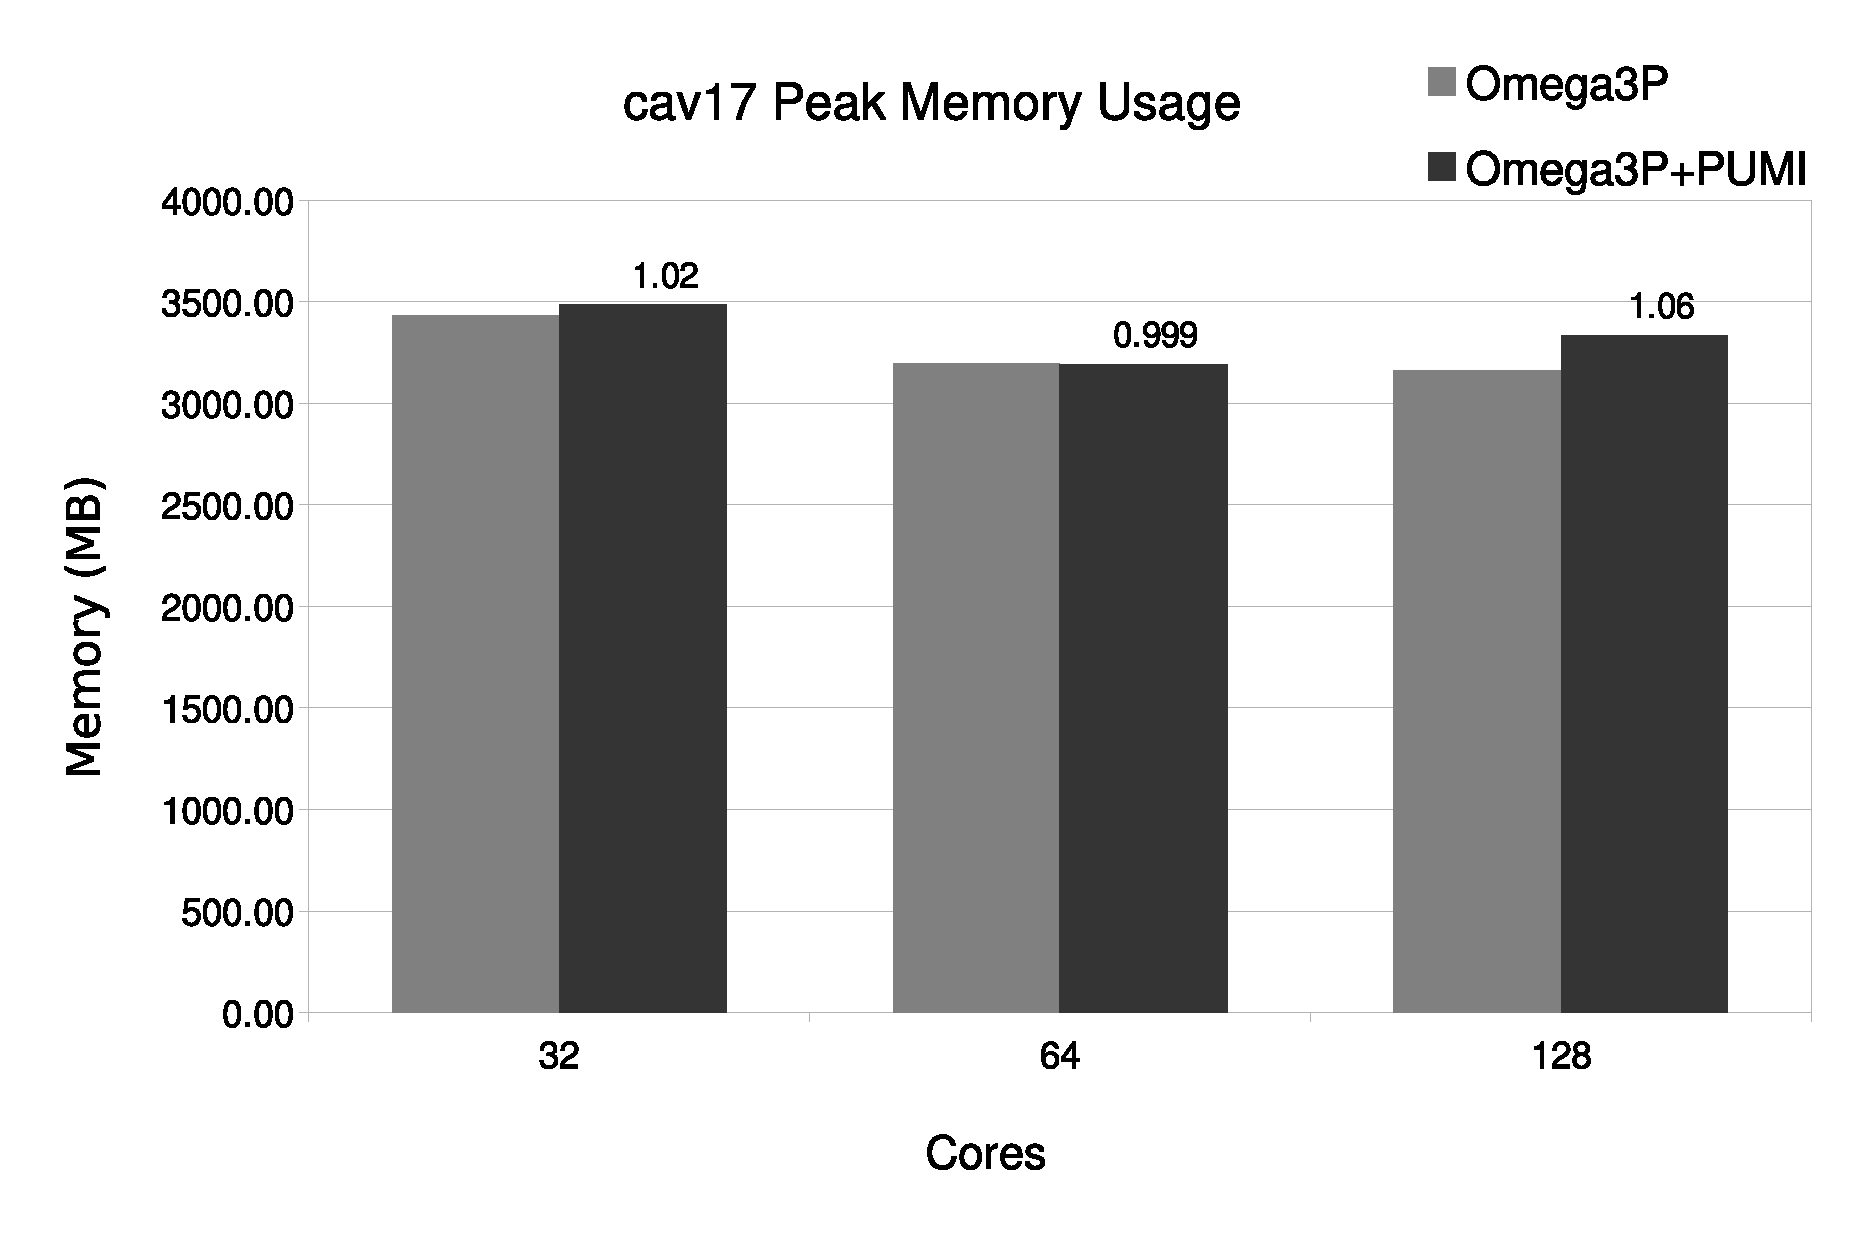
\includegraphics[width=.9\textwidth]{cav17-peak-mem.eps}
  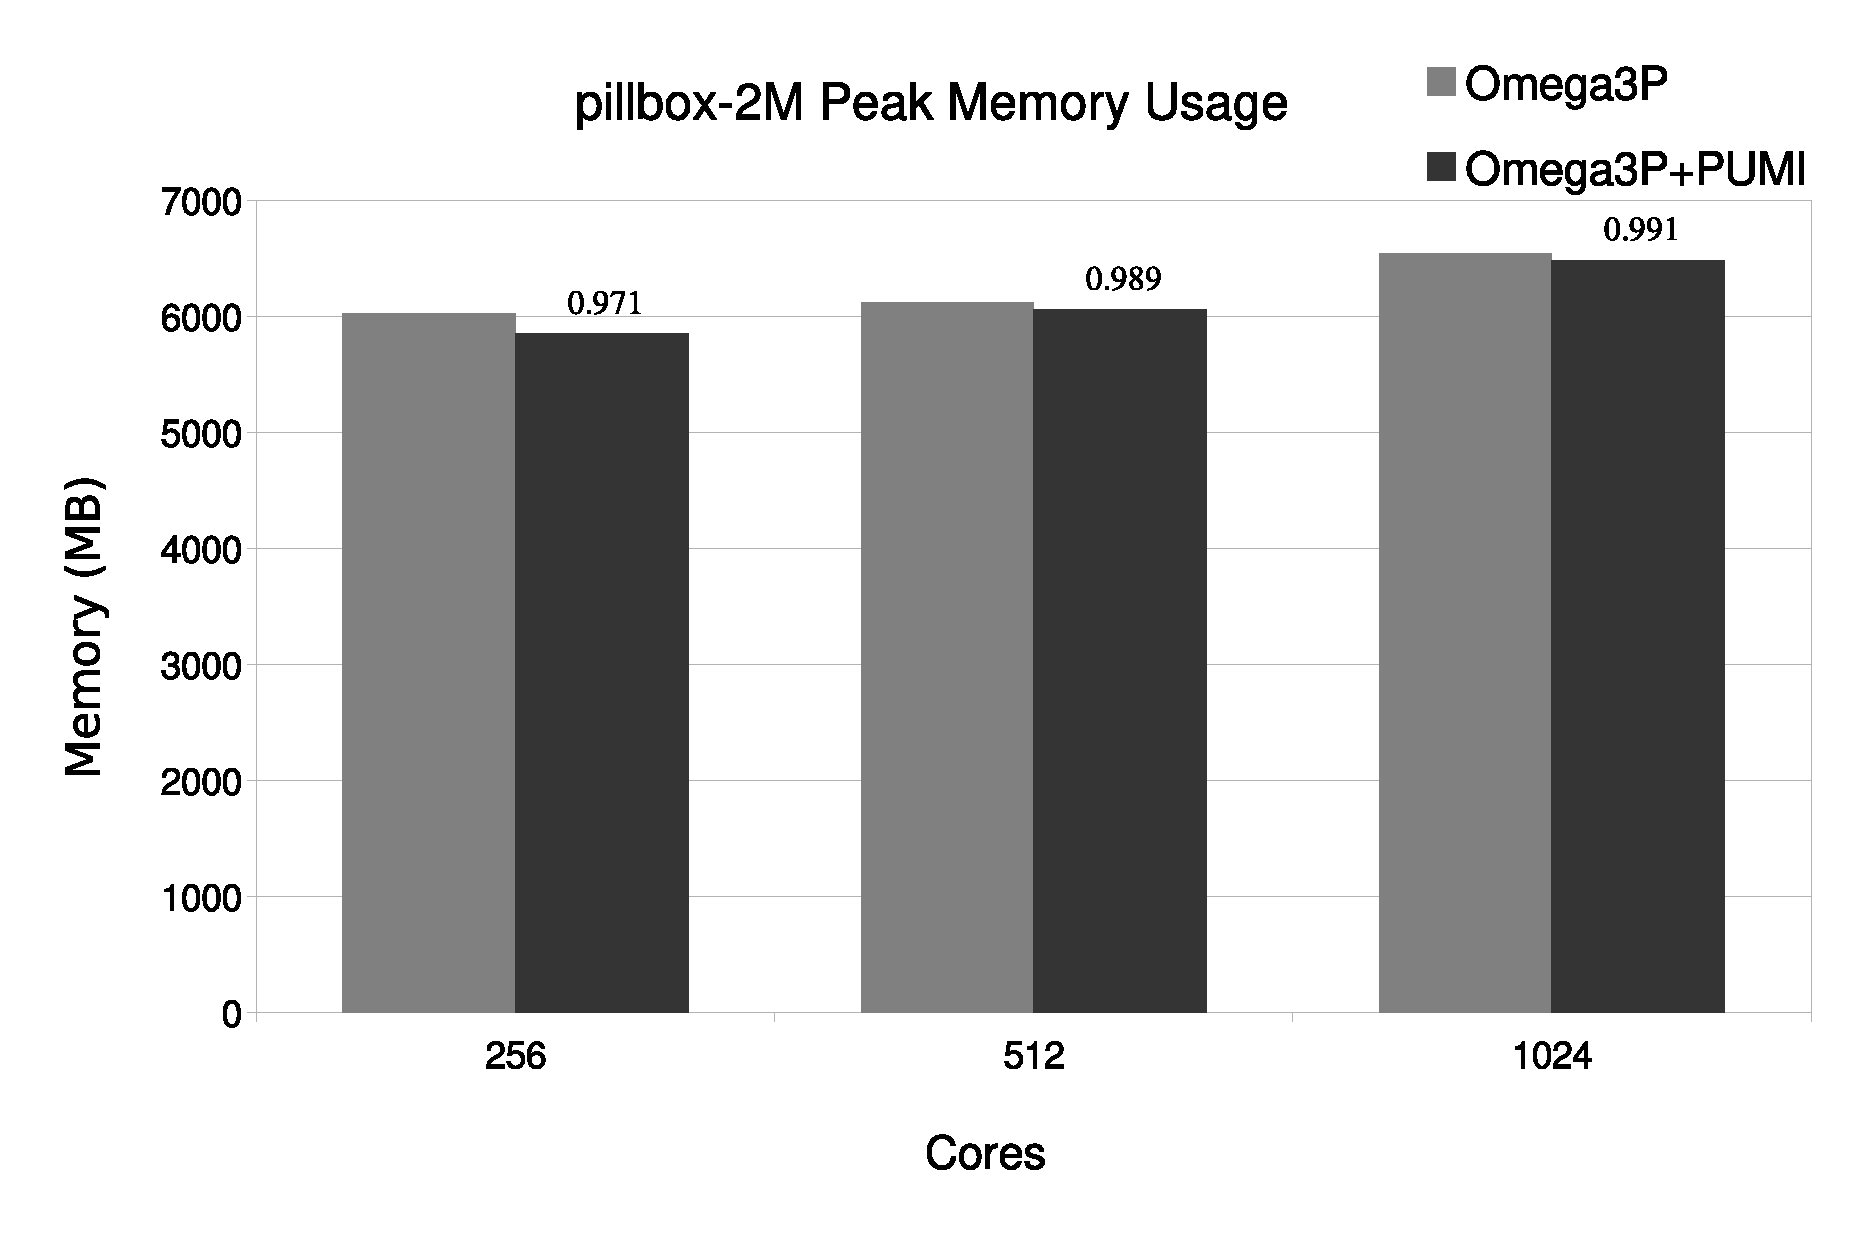
\includegraphics[width=.9\textwidth]{pillbox2M-peak-mem.eps}
  \caption{\label{fig:memusage} Peak memory usage. The labels above the Omega3P+PUMI bars
  list the percent increase versus Omega3P.}
\end{figure}

\subsection{\label{in_memory_future} Future Steps}
Our plan for future developments in regard to the in memory integration is as follows:

\setstretch{0.75}
\begin{itemize}
  \item item 1
  \item item 2
  \item \dots
\end{itemize}
\setstretch{1.5}

%Memory images to be added

\section{\label{load_balance}Load Balancing}
In each iteration of the mesh adaptation loop a new partition is generated on the
pumi-mesh before converted over to the slac-mesh. The initial partition is generated
using Zoltan's graph partitioning. Then SCOREC's ParMA, partitioning using mesh adjacencies,
is used to perform load balancing by iterative diffusion. ParMA's multi-entity balancing
traverses an application-specified priority list of entity orders (vertex, edge, face,
region) to balance in descending order.
For each entity order iterative diffusion is executed until balance is reached
or no further improvement is possible.

ParMA's support for multi-entity balancing was extended for Omega3P's needs.
The Omega3P solving step relies on both on-part mesh entities as well as a layer
of ghosted elements along each part boundary.
Omega3P's ghosting uses vertex adjacency such that every element that shares a
vertex with a part boundary will be ghosted to each part that shares that
boundary.
This can be seen in Figure \ref{fig:ghost3} that shows an example of a mesh with
a layer of ghosting.
In order to improve Omega3P's performance and scalability, ParMA targets
minimizing the sum of the ghosted and on-part elements as well as the mesh
entities holding degrees-of-freedom.

\begin{figure}[!ph]
\centering
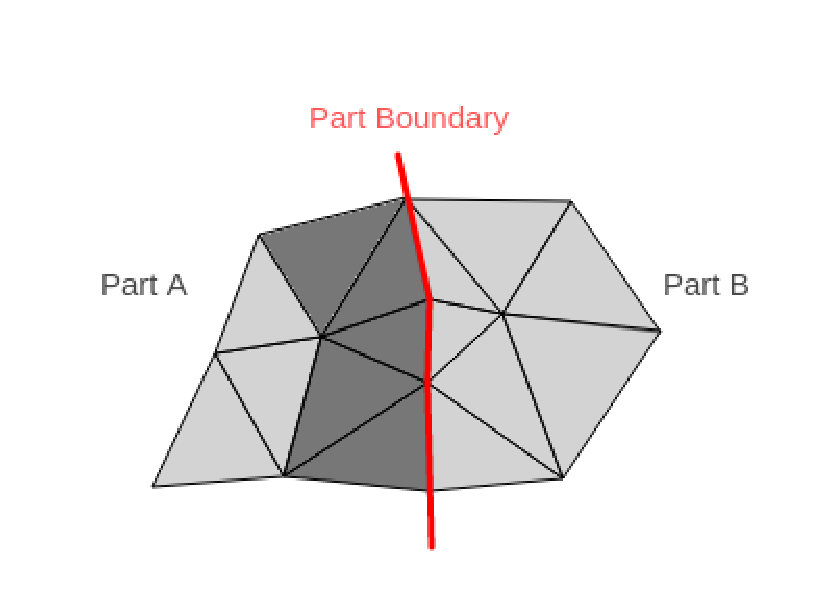
\includegraphics[width=0.6\textwidth]{ghost.eps} 
\caption{\label{fig:ghost3} A layer of ghosted elements from part A to part B. The darker elements represent all the elements on part A that part B will copy to create its remote mesh.}
\end{figure}

ParMA balances the degree-of-freedom holders defined by 
hierarchical Nedelec basis functions~\cite{ingelstrom2006new,ko2010advances} by
reusing existing multi-entity target and boundary-element selection
procedures.
For first order elements this requires balancing edges.
Second order elements requires edges and faces, and above that edges, faces, and
regions need to be balanced. \color{blue} Mark: Are we sure this is right? (I expect that is the case) \color{black}
Each of these entity balancing procedures accounts for the ghosted weight
contribution by performing an additional neighborhood
exchange~\cite{ibanez2014hybrid} of the exact weight of ghosted layer entities.
Thus ParMA can readily account for balancing the work load, in terms of number
of equations per-part, for p-version finite elements by setting mesh entity
weights based on the different entity p-orders. 

\subsection{\label{load_balance_results} Results}

We ran Omega3P and Omega3P with ParMA's ghost balances, from here on our referred
to as Omega3P+PUMI, on the \texttt{cav17} model with a 318,118
element quadratic mesh on up to 128 cores (32 cores per node) of the NERSC Cori
Phase I system.
The Omega3P+PUMI average number of ghost + owned edges and faces per-part
is less than 1.46\% higher than the Omega3P counts at 32 parts.
At 64 and 128 parts the average entity counts of Omega3P+PUMI is less than 0.3\%
higher than Omega3P counts.
While maintaining nearly identical entity counts ParMA significantly reduces the
imbalance of ghost + owned edges and faces degree-of-freedom holders.
Figure~\ref{fig:cav17imb} shows the imbalance of edges and faces.
At 128 parts ParMA reduces the edge imbalance by 30 points and the face
imbalance by 27 points.
At 64 parts the edge and face imbalances are reduced by over 15 points each and
at 32 parts ParMA reduces the imbalances by eight points.

\begin{figure}[!ph]
\centering
  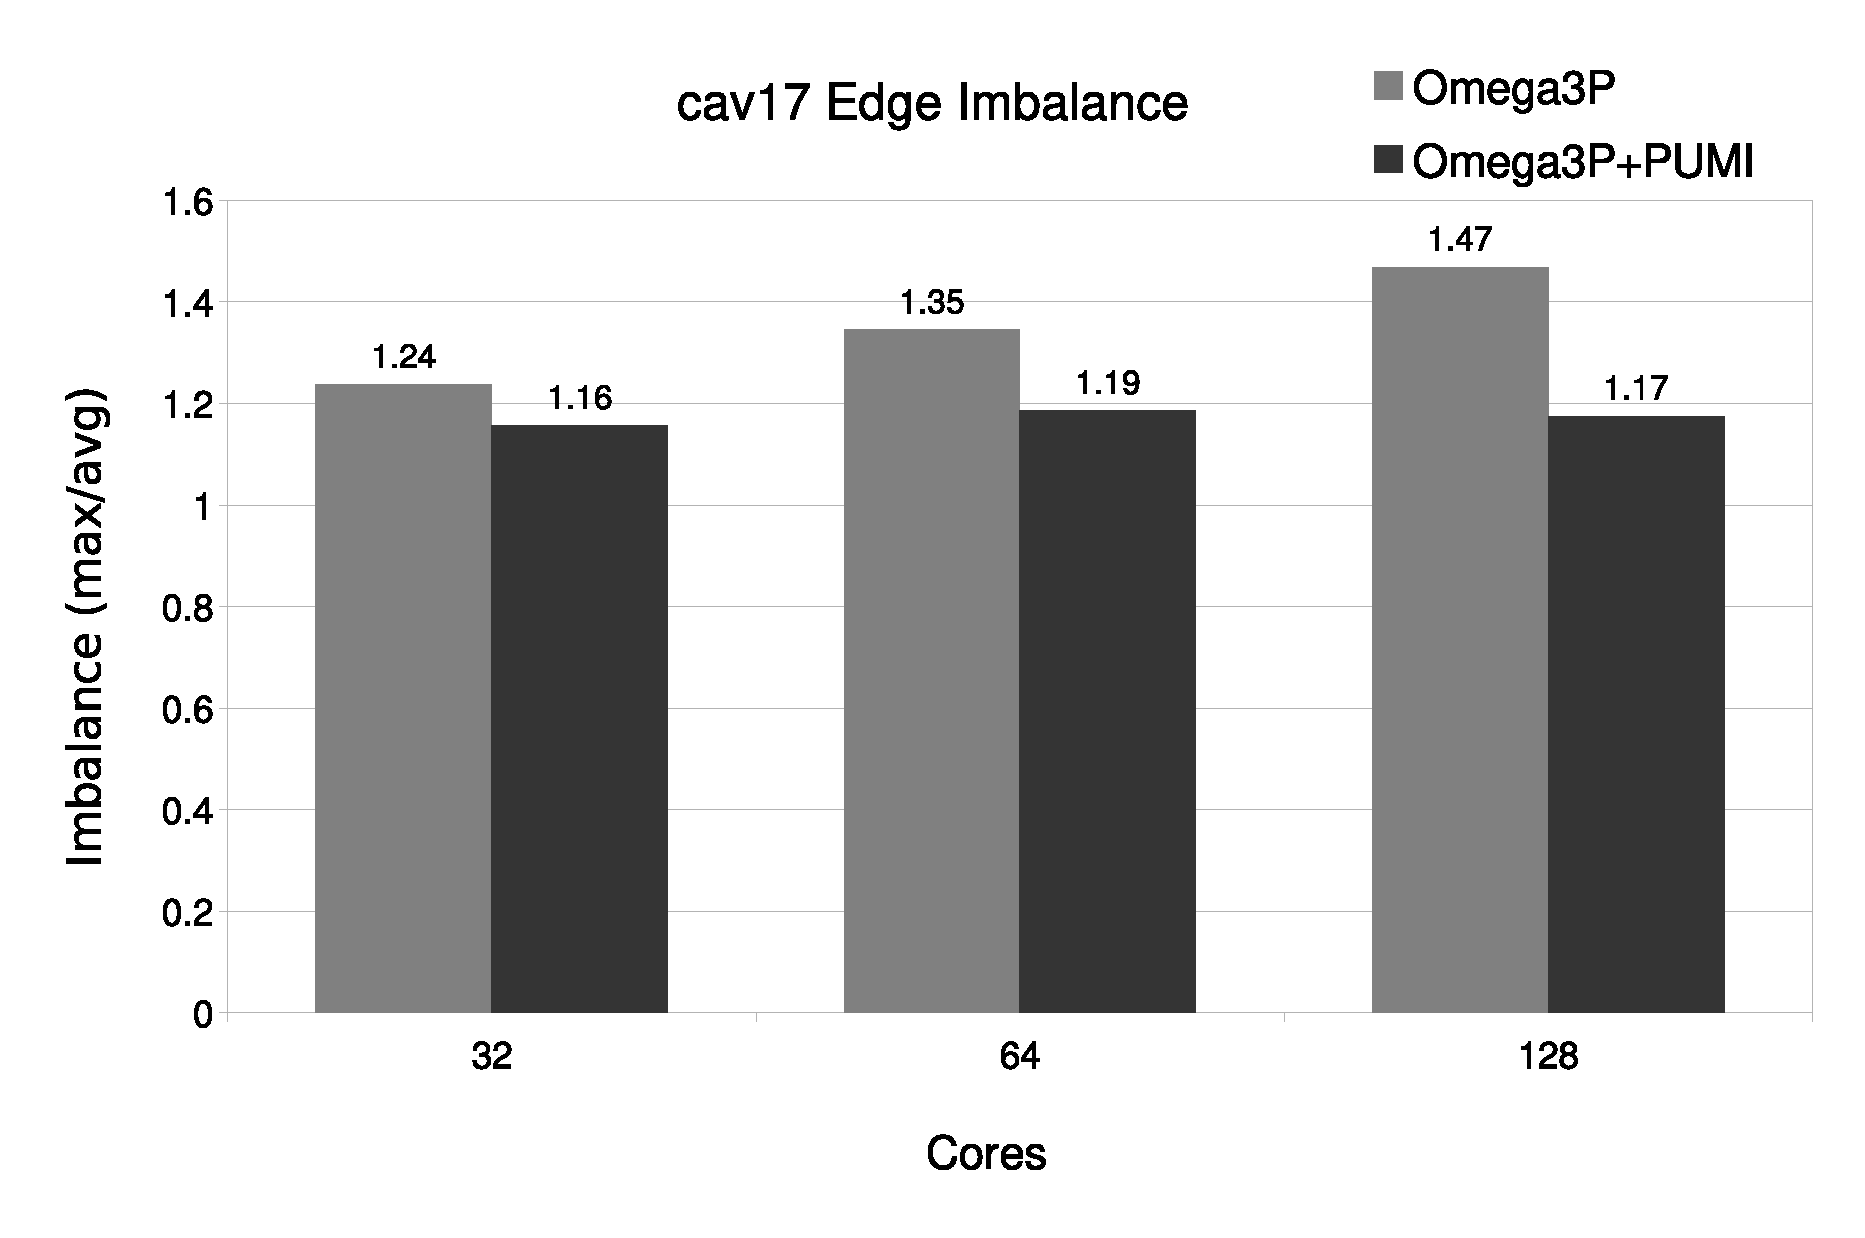
\includegraphics[width=0.75\textwidth]{cav17-edge-imb.eps} \\
  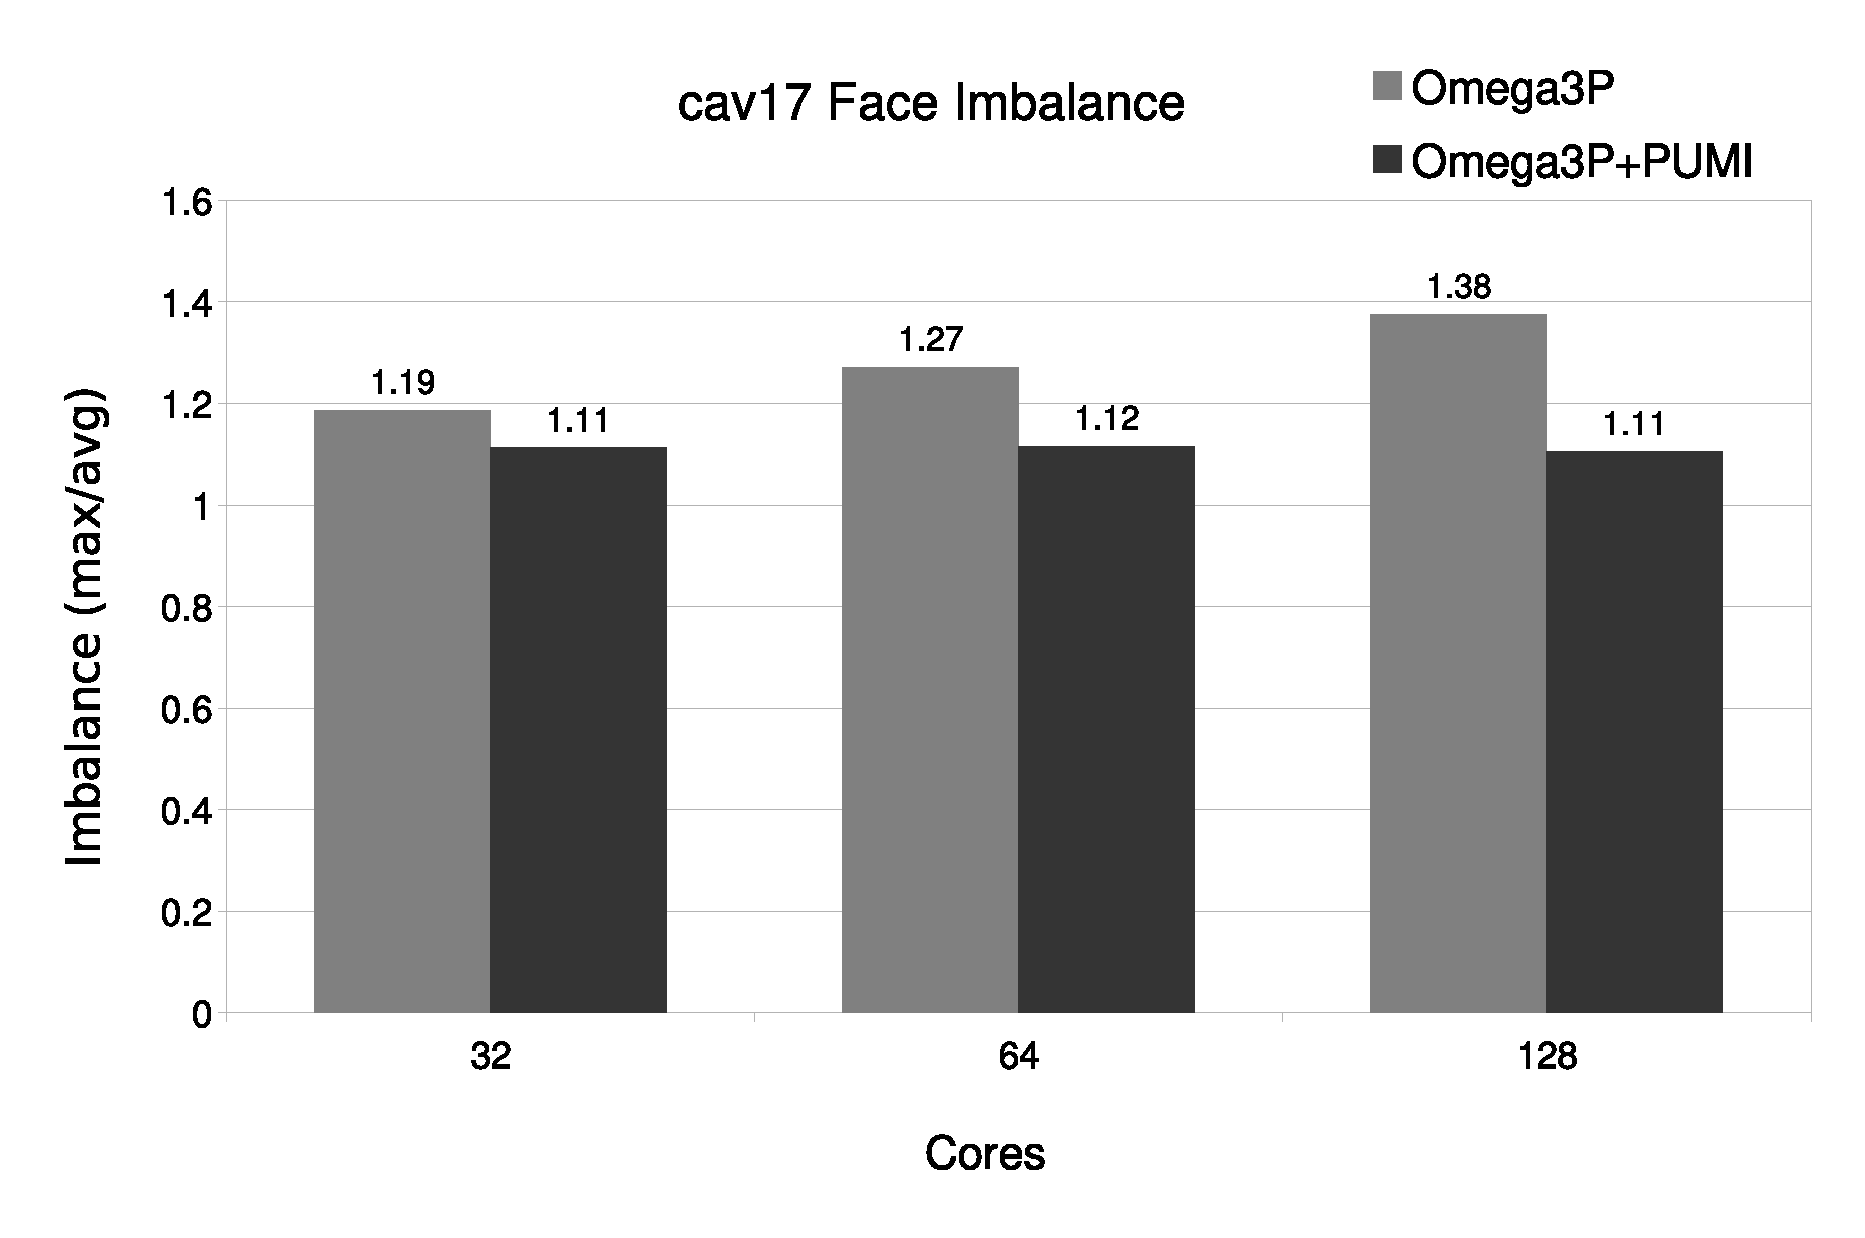
\includegraphics[width=0.75\textwidth]{cav17-face-imb.eps} 
  \caption{\label{fig:cav17imb} Edge and face imbalance in the {\texttt cav17} mesh.}
\end{figure}

Additional tests of ParMA ghost-aware edge balancing were executed on the
\texttt{pillbox} model with a 2 million element quadratic mesh on up to 1024
cores (32 cores per node) of the NERSC Cori Phase I system.
The Omega3P+PUMI average number of ghost + owned edges and faces per-part
is less than 1.15\% higher than the Omega3P counts at 256, 512, and 1024 parts.
With this insignificant increase in entity count ParMA reduces the imbalance of 
ghost + owned edges and faces by over 50 points.
At 1024 parts Figure~\ref{fig:pillboximb} depicts the ParMA reduction of the
edge imbalance by 55 points and the face imbalance by 48 points.
At 512 parts the edge and face imbalances are reduced by over 40 points each and
at 256 parts ParMA reduces the imbalances by over 25 points.
These reductions to the degree-of-freedom holding entities have been
demonstrated to significantly improve the performance and scalability of
parallel finite element simulations~\cite{zhou2012unstructured}.


\begin{figure}[!ph]
\centering
  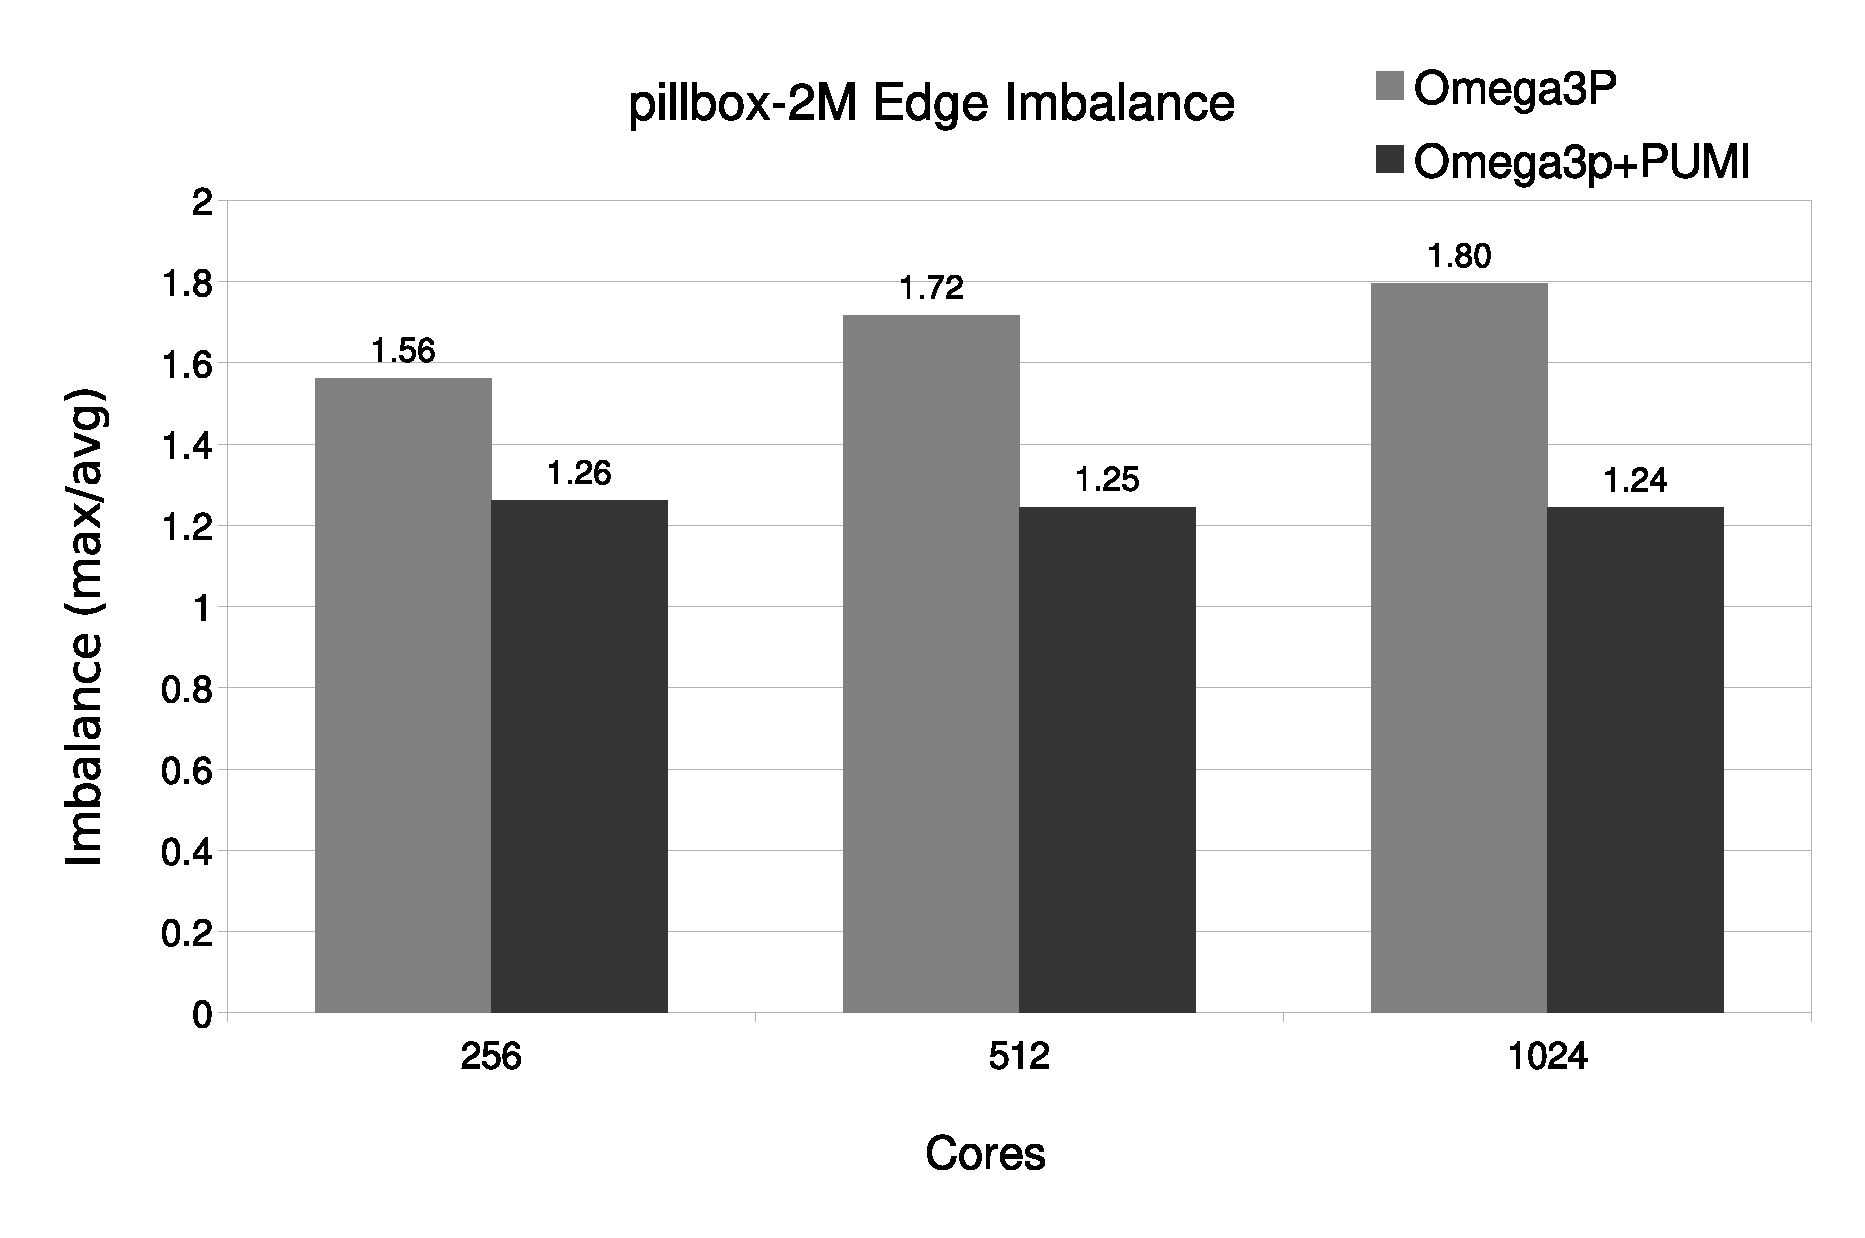
\includegraphics[width=0.75\textwidth]{pillbox2M-edge-imb.eps} \\
  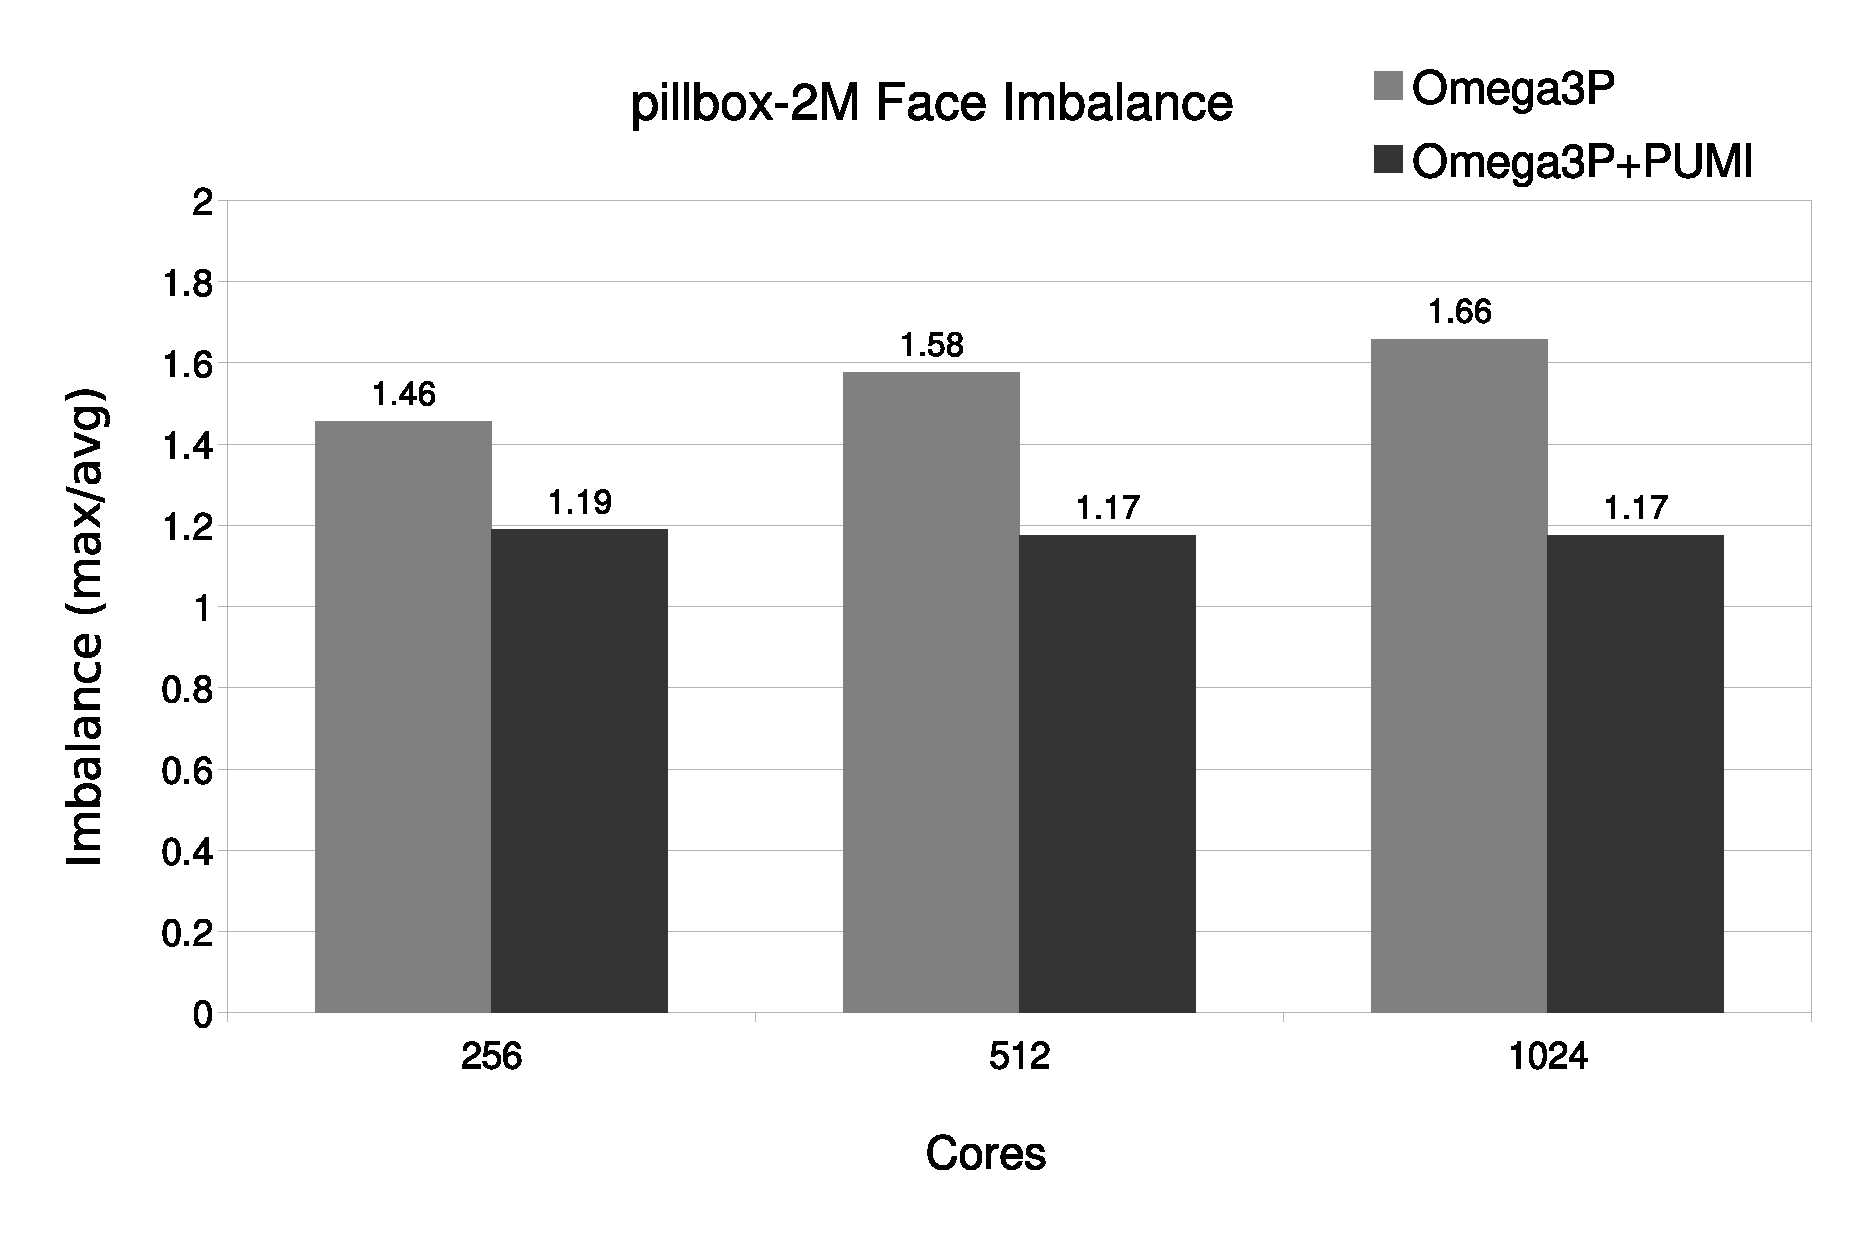
\includegraphics[width=0.75\textwidth]{pillbox2M-face-imb.eps}
  \caption{\label{fig:pillboximb} Edge and face imbalance in the {\texttt
  pillbox-2M}
  mesh.}
\end{figure}

\subsection{\label{load_balance_future} Future Steps}
While we have seen major improvements in the degree of freedom holder imbalance,
we have yet to see an improvement in runtime as a result of the balancing. Thus
our plan for future developments in regard to the load balancing  is as follows:

\setstretch{0.75}
\begin{itemize}
  \item Determine how the distribution of degrees of freedom effects the runtime for Omega3P.
  \item Further optimize the ParMA ghost balancer to improve runtime of Omega3P solvers.
\end{itemize}
\setstretch{1.5}


% \clearpage
% \newpage

\section{\label{adaptive_loop}The Adaptive Loop}
At this stage, we have the adaptation loop in place which consists of the following steps:

\setstretch{0.75}
\begin{itemize}
  \item[] \texttt{while not converged \{ }
   \begin{itemize}
     \item \texttt{partition the mesh using ParMA with a focus of owned and ghost elements}
     \item \texttt{convert PUMI-mesh to SLAC-mesh}
     \item \texttt{run the appropriate Omega3P eigensolver}
     \item \texttt{transfer electric field values to the PUMI-mesh}
     \item \texttt{check for convergence}
     \item \texttt{run Super-convergent Patch Recovery (SPR) -> error estimation -> size field}
     % \item \texttt{convert 2nd order Lagrange to 2nd order Bezier}
     \item \texttt{run the curve adapt} % \color{red} What about (1)predictive load balancing (2) re-balancing before solve, etc \color{black}
     % \item \texttt{convert 2nd order Bezier back to 2nd order Lagrange}
   \end{itemize}

 \item[] \texttt{  \} }
\end{itemize}
\setstretch{1.5}

The curve adapt step in the above loop involves more details that are explained next.
\setstretch{0.75}
\begin{itemize}
  \item [1.]In order to be able to use the curve adapt tools in Pumi we first need to convert the mesh to a quadratic Bezier mesh (currently curve adapt in PUMI only supports Bezier meshes).
  \item [2.]The actual curve adapt step involves the following operations
  	\begin{itemize}
	  \item \texttt{pre-adapt balancing of the mesh}
	  \item \texttt{coarsening the mesh based on the size-field}
	  \item \texttt{mid-adapt balancing of the mesh}
	  \item \texttt{refining the mesh base on the size-field}
	  \item \texttt{post-adapt balancing of the mesh}
  	\end{itemize}
  \item [3.]After the adaptation is done we convert the mesh back to Lagrange quadratic.
\end{itemize}
\setstretch{1.5}

It is important to note that the coarsening and refinement steps are done with snapping functionality (i.e., the newly created vertexes and Bezier interpolating points will be snapped to the corresponding model entities that they are categorized on). 


Also worth mentioning, is the fact that our current pipeline works with PUMI-meshes as an input without the need for an input NETCDF mesh. This enables us to generate our initial meshes using Simmetrix. Note that the current geometric model inquiries for the purpose of snapping the vertex and mid-edge nodes to the model, requires Simmetrix.

Finally,  the current adaptive loop improves upon the previously available adaptive loop (implemented by Kai) in that it is fully parallel. Recall that the previous implementation required repartitioning a serial mesh after parallel adaptation.

\subsection{Results for the Adaptive Loop}

\color{blue} Mark: The mesh adaptation procedures are currently doing what looks like a poor job on creating the new mesh topology. This is something we will want to work on when we can get to it. (will likely (1) be a while before we can get to it, (2) take a fair amount of work) \color{black}

\color{blue} Mark: on subfigures (b) and (d): Why are we plotting such different things? We want the same simulation fields on both. \color{black}


Figures \ref{pill} and \ref{cav} show two working examples for the current curve adaptation loop.
In particular, Fig. \ref{pill} shows the results for the smaller ``PILLBOX''. We start with a uniform and relatively coarse mesh as shown in Fig. \ref{pill_init}. The desired size field for this initial mesh is obtained based on the magnitude of the electric filed and it is shown in Fig. \ref{pill_size}. The final, adapted mesh (for this specific example we needed 3 levels of adaptation) is shown in Fig. \ref{pill_adapt}. Figure \ref{cav} shows the corresponding result for the larger ``CAV17'' model. \color{blue} Mark: More technical Info \color{black}
\begin{landscape}
\begin{figure}[ph!]
\centering
\subfigure[]{\label{pill_init}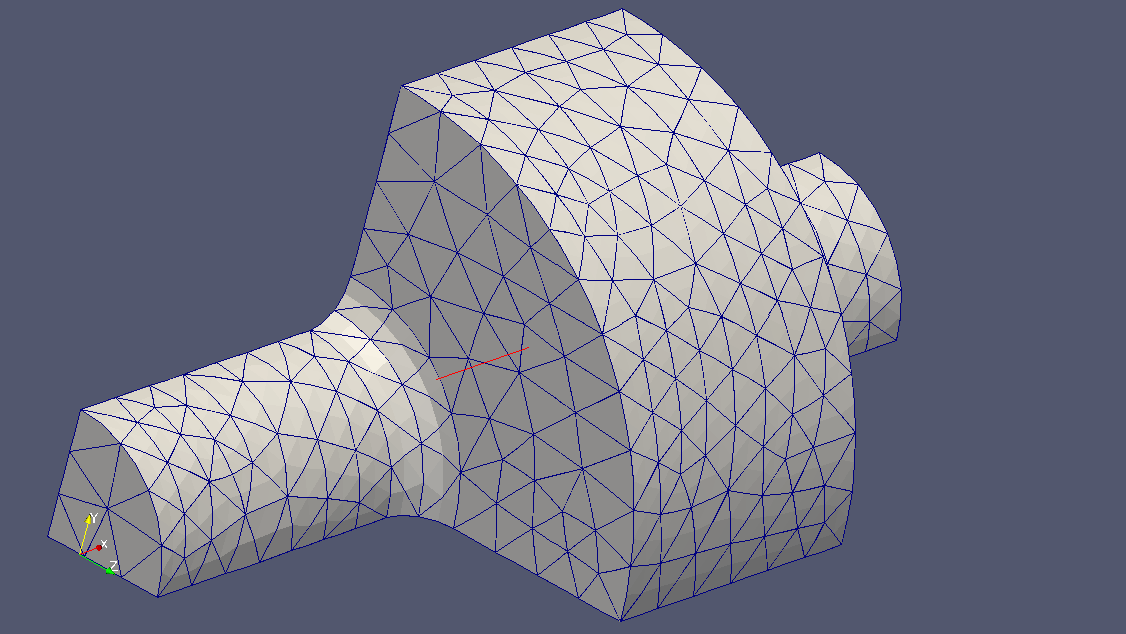
\includegraphics[width=0.55\textwidth]{al_0_ar_0p0125_3721_elems.png}}
\hspace*{50pt}
\subfigure[]{\label{pill_size}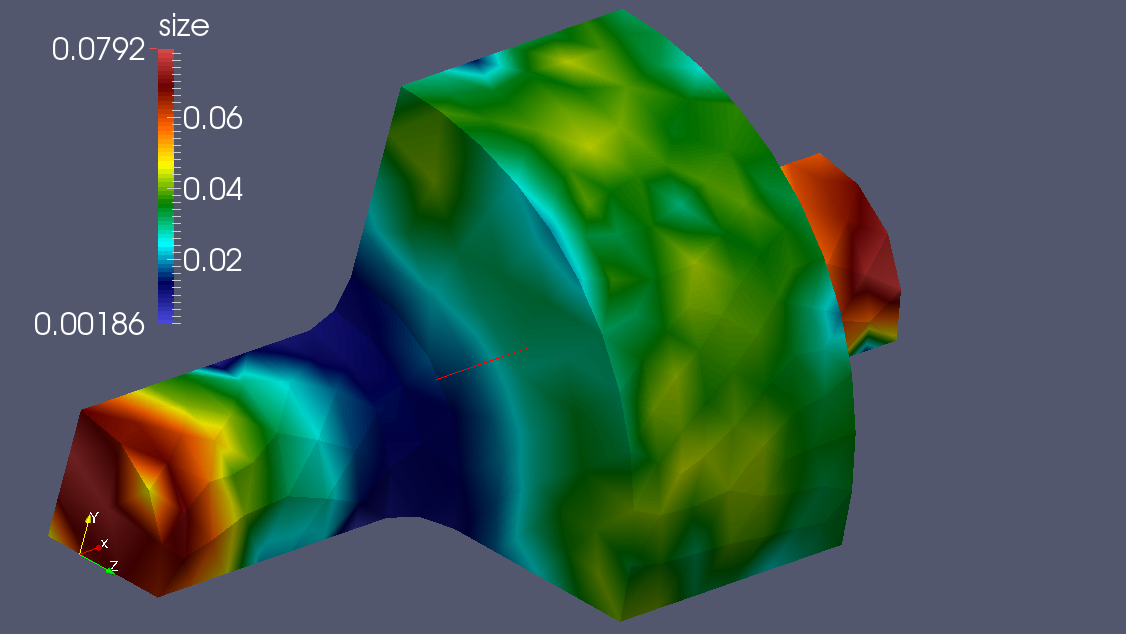
\includegraphics[width=0.55\textwidth]{al_0_ar_0p0125_3721_elems_size_field.png}}
\\
\subfigure[]{\label{pill_adapt}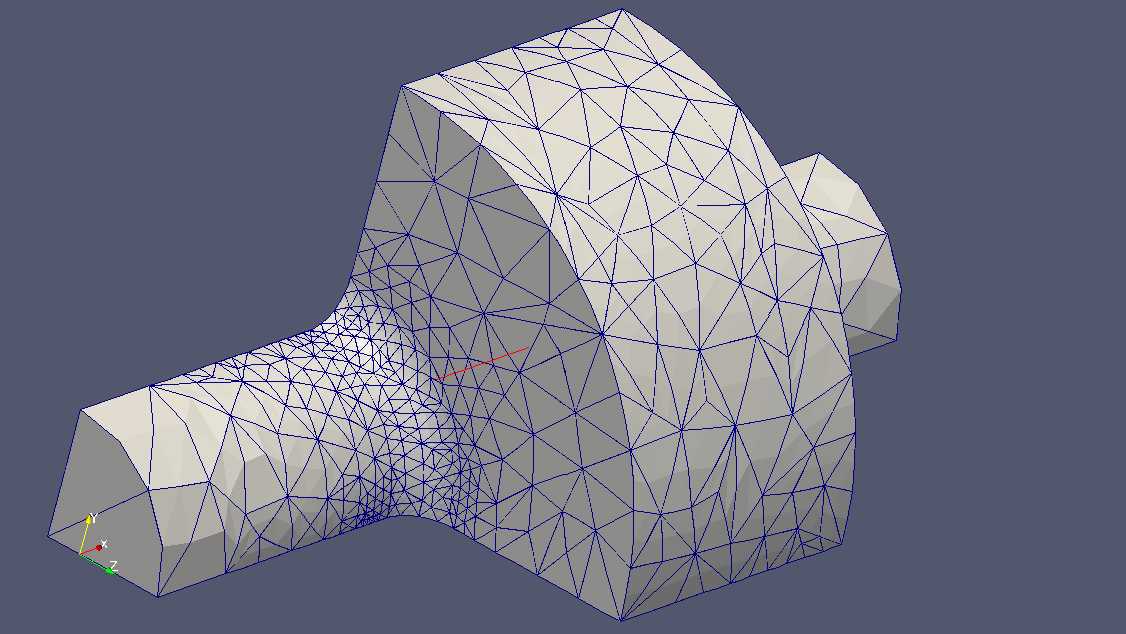
\includegraphics[width=0.55\textwidth]{al_3_ar_0p0125_14221_elems.png}}
\hspace*{50pt}
\subfigure[]{\label{pill_field}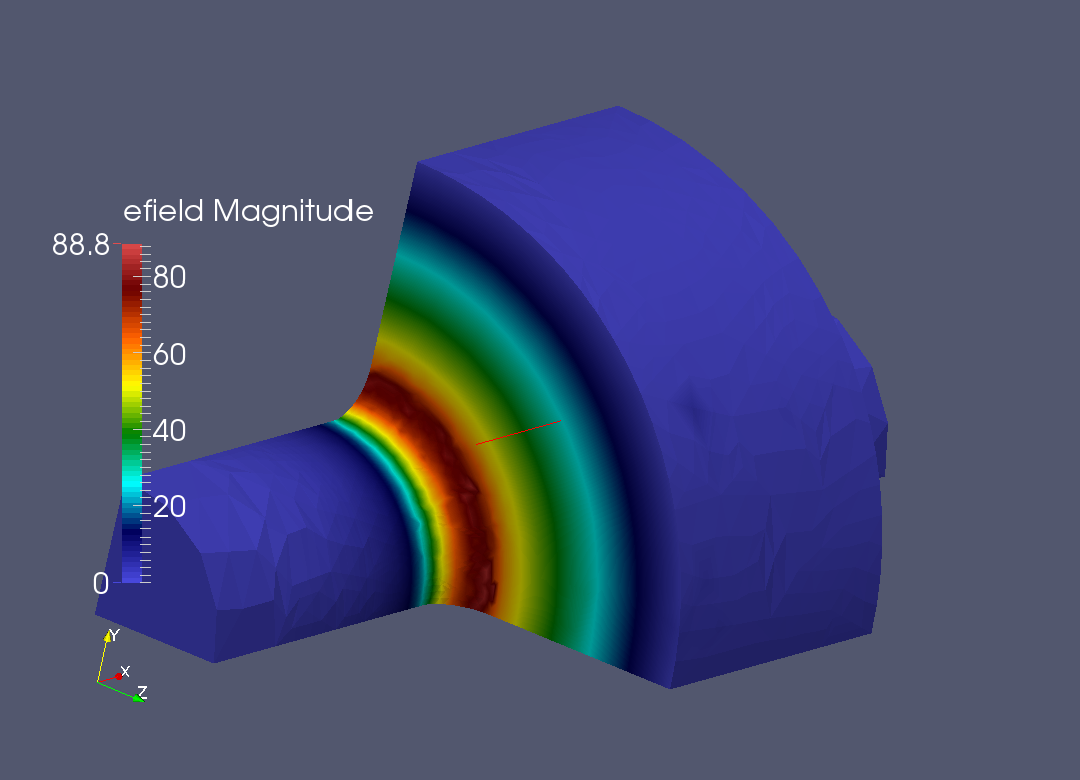
\includegraphics[width=0.55\textwidth]{al_3_ar_0p0125_14221_elems_e_field.png}}
\caption{\label{pill} This Figure shows the results for the PILLBOX model. (a) shows the initial mesh [$\sim3.7\text{K}$ elements], (b) shows the initial size-field, (c) shows the adapted mesh after 3 adaptation steps [$\sim14\text{K}$ elements], and (d) shows the electric field for the final adapted mesh.}
\end{figure}
\end{landscape}
\begin{landscape}
\begin{figure}[ph!]
\centering
\subfigure[]{\label{cav_init}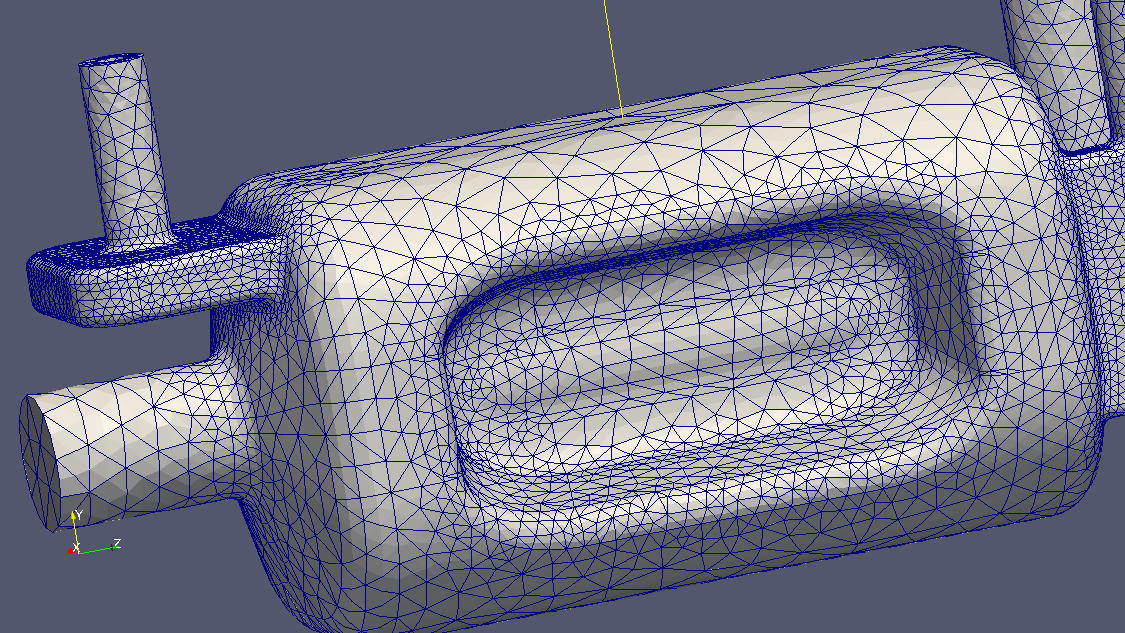
\includegraphics[width=0.55\textwidth]{al_0_ar_0p0125_126044_elems.png}}
\hspace*{50pt}
\subfigure[]{\label{cav_size}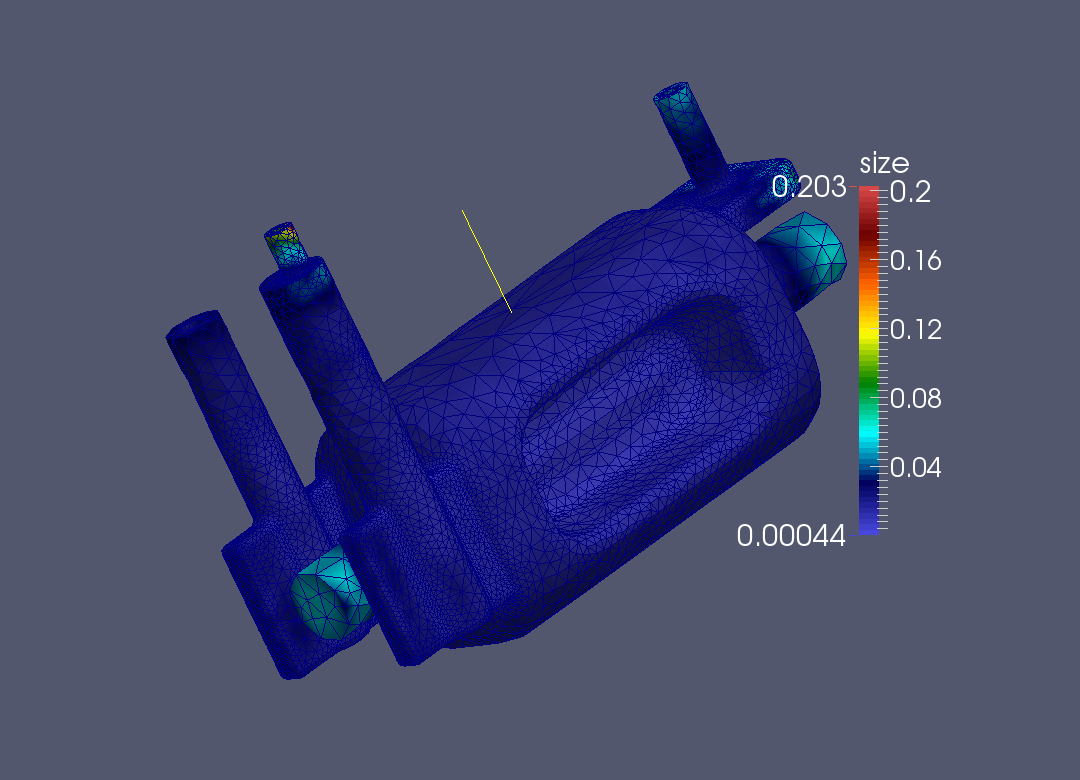
\includegraphics[width=0.55\textwidth]{al_0_ar_0p0125_126044_elems_size_field.png}}
\\
\subfigure[]{\label{cav_adapt}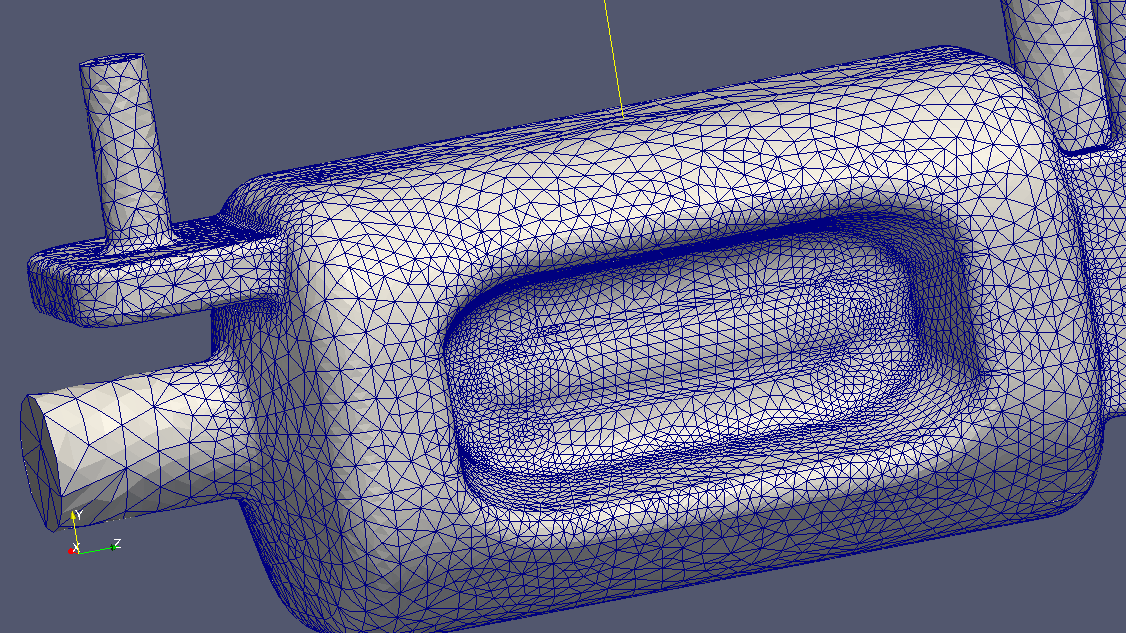
\includegraphics[width=0.55\textwidth]{al_3_ar_0p0125_386896_elems.png}}
\hspace*{50pt}
\subfigure[]{\label{cav_field}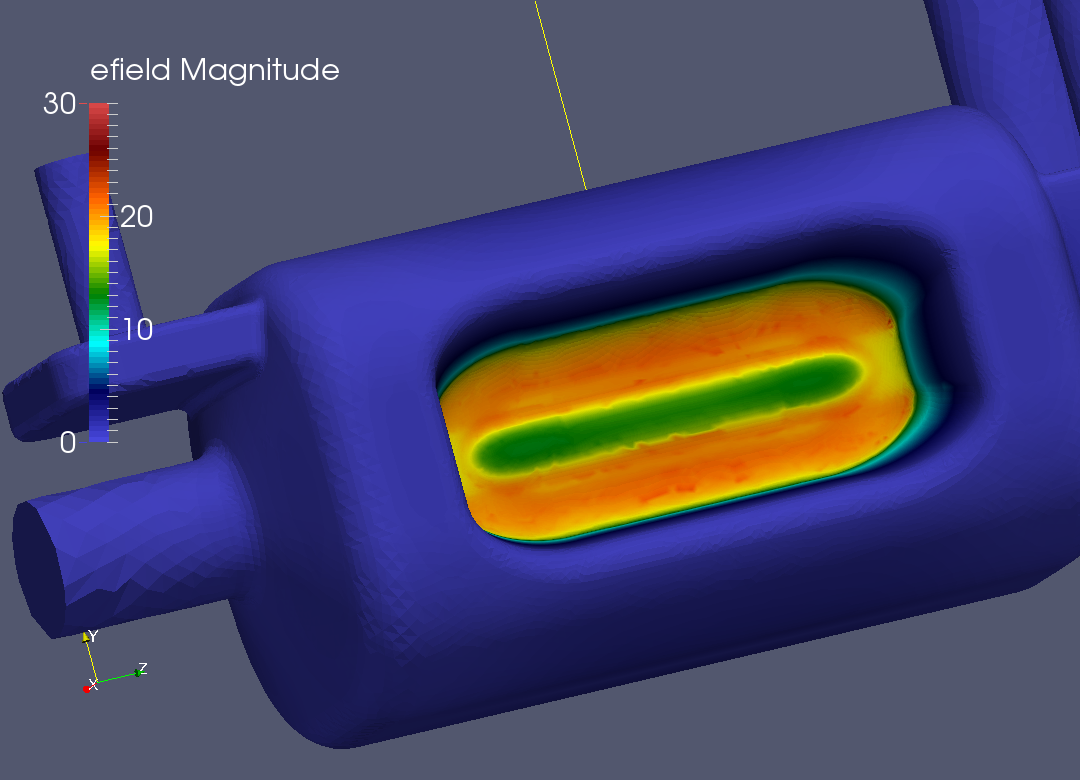
\includegraphics[width=0.55\textwidth]{al_3_ar_0p0125_386896_elems_e_field.png}}
\caption{\label{cav} This Figure shows the results for the CAV17 model. (a) shows the initial mesh [$\sim126\text{K}$ elements], (b) shows the initial size-field, (c) shows the adapted mesh after 3 adaptation steps [$\sim380\text{K}$ elements], and (d) shows the electric field for the final adapted mesh.}
\end{figure}
\end{landscape}
\subsection{\label{adaptive_loop_future} Future Steps}

Our plan for future developments in regard to the adaptive loop is as follows:
\setstretch{0.75}
\begin{itemize}
  \item to be completed
  \item \dots
\end{itemize}
\setstretch{1.5}



\section{\label{high_order_geom}Moving Towards Higher-Order Geometries}

In order to be able to increase the order of the finite element basis functions to exploit the exponential convergence rate of the p-version finite elements, one needs to also increase the geometric order of the elements near the curved boundaries. Otherwise, the error in the geometric representation of such curved elements prevents the exponential growth rate in the p-version finite element \cite{LuoShephard_04, DeyShephard_97, LuoShephard_02}.

The finite element discretization of the problem involves volume integrals of the form \cite{LeeLi_09}
\begin{equation}
  \int _\Omega \pr{D \textbf{N}^i} \cdot \pr{D \textbf{N}^j} d\Omega \quad \quad \text{or} \quad \quad \int _{\Omega _e} \pr{D \textbf{N}^i} \cdot \pr{D \textbf{N}^j} d\Omega _e	
  \label{integrals}
\end{equation}
where $\Omega$ and $\Omega _e$ denote the whole domain of the problem  and the element volume, respectively, and the operator $D$ is either of the following two operators 
\begin{equation}
  D \in \cbr{\textbf{I}, \nabla \times }.
\end{equation}
The element integrals in \mref{\ref{integrals}}{2}, can then be re-written with respect to the parametric coordinates in the reference element, e.g., the stiffness matrix for each element can be written as follows
\begin{equation}
\begin{aligned}
  K^{ij} 	&= \int _{\Omega _e} \pr{\nabla _x \times \textbf{N}^i} \cdot \pr{\nabla _x \times \textbf{N}^j} d\Omega _e \\
  &= \int _{\Omega _e} \epsilon _{kmn} \epsilon_{kpq} \frac{\partial N^i_m}{\partial x_n} \frac{\partial N^j_p}{\partial x_q}   d\Omega _e \\
  &= \int _{\Omega _\xi} \epsilon _{kmn} \epsilon_{kpq} \frac{\partial N^i_m}{\partial \xi_s} \frac{\partial \xi_s}{\partial x_n}  \frac{\partial N^j_p}{\partial \xi_t}  \frac{\partial \xi_t}{\partial x_q} \abs{\frac{\partial x}{\partial \xi}  } d\Omega _\xi \\
  &= \int _{\Omega _\xi} \epsilon _{kmn} \epsilon_{kpq} \frac{\partial N^i_m}{\partial \xi_s} J^{-1}_{sn}  \frac{\partial N^j_p}{\partial \xi_t}  J^{-1}_{tq} \abs{J} d\Omega _\xi.
\end{aligned}
\end{equation}
Here $\epsilon_{kmn}$ is the third-order permutation tensor, and $N^i$ are the shape functions. Assuming that the Omega3P's code for the computation of the stiffness matrix (or any other matrix pertaining the fem discretization) does not make any specific assumption on the choice of the shape functions, we can safely use other valid shape functions, and  achieve a valid fem discretization. Note that the geometric information of each element is encapsulated in the Jacobians appearing in the above integral, and therefore incorporating higher order geometries into the finite element formulations requires the computation of the Jacobian for higher order elements.  

As a first step towards using higher-order geometric elements, we have been able to replace the Omega3P calls to compute the Jacobian-related quantities (e.g., the determinant) with the corresponding PUMI calls. This is done by storing an additional pointer in each Omega3P-element that points to the corresponding  PUMI-element (see Fig. \ref{imp} for the details of the implementation).
\begin{figure}[ph!]
\centering
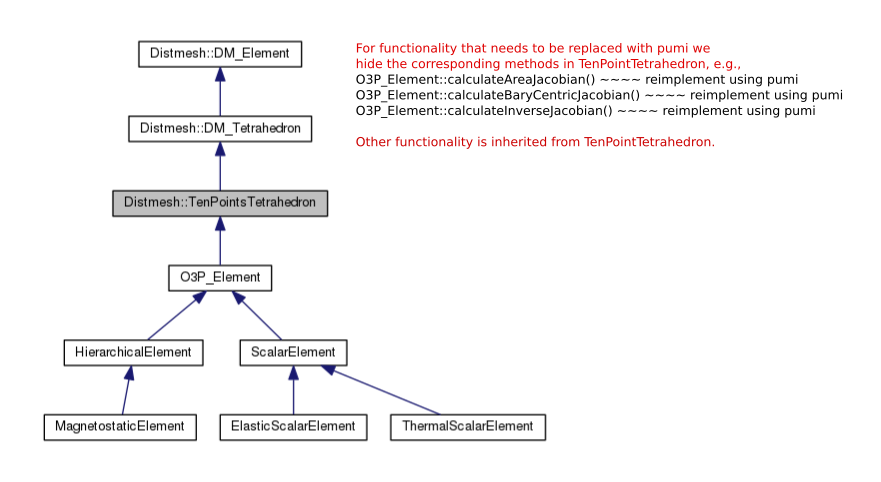
\includegraphics[width=0.95\textwidth]{hide_ten_point_tet.png}
\caption{\label{imp} This Figure shows the implementation details for replacing Omega3P calls for determinant calculation with the corresponding PUMI calls.}
\end{figure}
This enables us to easily redirect any call in Omega3P that requires the Jacobians to PUMI and retrieve the corresponding value using the PUMI Jacobian calculations, which supports higher than quadratic geometries. (Currently, we have support for up to 6th order Bezier elements in PUMI.)


\subsection{\label{high_order_geom_future} Future Steps}
By replacing the Jacobian calls in Omega3P with the corresponding PUMI calls we were able to pass the current tests for meshes with quadratic curved  elements, and therefore demonstrate that the above approach works. Our plan for future developments in regard to the higher-order geometries is as follows:

\setstretch{0.75}
\begin{itemize}
  \item Move to higher order finite element with support for higher order geometries using the approach described above
  \item Once we have full support for higher order geometries we plan to compare the performance improvements of p-version finite element with that of the h-version finite element. 
\end{itemize}
\setstretch{1.5}

\section*{References}
% \bibliographystyle{elsarticle-harv_noURL}
\bibliographystyle{plain}
\bibliography{scorec-refs/partition,scorec-refs/meshdb,scorec-refs/hardware,scorec-refs/io,scorec-refs/frameworks,scorec-refs/cr,scorec-refs/fem,scorec-refs/meshgen,scorec-refs/msgpass,geometry}


\end{document}
